\styledchapter[Stappen in een Machine Learning pipeline]{stappen-in-een-machine-learning-pipeline}

Een ML pipeline is zoals beknopt beschreven in \autoref{subsec:opzetten-pipeline} een collectie van stappen dat wordt doorlopen om een model te trainen. Elke stap bevat een aantal acties dat wordt uitgevoerd, zoals onbruikbare data weghalen of de prestatie analyseren. De stappen en acties wordt in \autoref{sec:de-stappen-met-een-praktisch-voorbeeld} uitgelegd. Een van de stappen in een pipeline is het trainen van het model. Om een idee te krijgen van ML en modellen trainen wordt dit kort uitgelegd.

\section{Wat is machine learning?}\label{sec:wat-is-machine-learning}
ML houdt in dat een computer een taak kan uitvoeren zonder ervoor expliciet geprogrammeerd te zijn. Dit wordt gedaan door een ML model te laten leren van een gegeven dataset. Vervolgens kan er een voorspelling worden gemaakt \cite[p.~1-3]{introduction-to-machine-learning}.

De domeinen deep learning (DL), neural networks (NN) en artificial intelligence (AI) komen vaak voor als het over ML gaat. Zoals weergegeven in \autoref{fig:ai-ml-nn-dl} is te zien dat ML een subset is van AI, NN een subset van ML en als laatste DL dat een subset is van NN.

Bij AI wordt niet alleen ML toegepast, maar ook concepten zoals beredeneren, plannen, vooruitdenken, onthouden en terug refereren. Een voorbeeld hiervan is dat een ML model kan voorspellen wat het volgende woord in een zin kan zijn, maar een AI kan beredeneren waarom de zin gebouwd is zoals het is en hoe het binnen de context van de alinea past \cite{ml-think-about-ml-brownlee}.

\begin{figure}[hbt!]
  \centering
  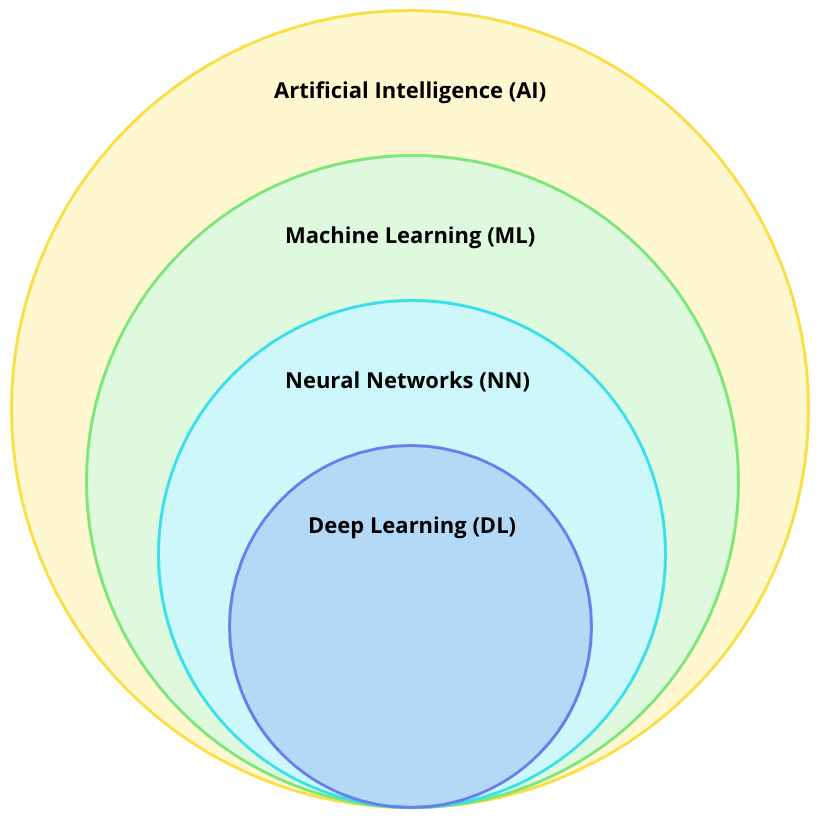
\includegraphics[width=0.48\textwidth]{chapter-4/AI-ML-NN-DL.png}
  \caption{Machine learning in de context van andere domeinen}
  \label{fig:ai-ml-nn-dl}
\end{figure}

Een NN bestaat uit een collectie van nodes dat gemodelleerd is naar de hersenen. Een NN heeft minimaal 3 lagen: een input laag, een verborgen laag en een output laag. Elke laag bevat neuronen dat data als input kan krijgen en data als output aan de volgende laag meegeeft. DL is een NN dat meerdere verborgen lagen bevat \cite{ml-neural-network-nicholson}.

In het ML domein bestaan talloze algoritmes om voorspellingen te maken. In de [BIJLAGE LINK] is een mind-map te vinden van de algoritmes die gedurende de scriptie naar voren zijn gekomen. Het grotendeels kan gegroepeerd worden in vier stijlen: supervised, unsupervised, semi-supervised en reinforcement learning. In de [BIJLAGE LINK] is meer informatie over de stijlen te vinden.

Het trainen van een model is een proces waarbij vooraf data wordt opgeschoond en achteraf de prestatie van het model wordt gevalideerd. Normaliter wordt dit gedaan door specifieke code te schrijven voor deze taken. Een valkuil is dat de code niet bij elke developer werkt en schaalt niet in alle gevallen naar een productie omgeving. Een manier om dit wel te behalen is om te werken met ML pipelines. Zoals kort uitgelegd in \autoref{subsec:opzetten-pipeline} bestaat een ML pipeline uit stappen en acties. Er is echter geen consensus binnen het ML domein over wat de juiste stappen en acties in een pipeline zijn. Voor de scriptie is gekozen voor een pipeline van Hapke en Nelson uit het boek "Building Machine Learning Pipelines". Het boek is gemaakt en gepubliceerd door O'Reilly; een bekend en gecrediteerd bedrijf dat boeken maakt binnen het software engineering domein.

\section{De stappen in een machine learning pipeline}\label{sec:de-stappen-in-een-machine-learning-pipeline}
Een ML pipeline begint met het opnemen van data en eindigt met het ontvangen van feedback om de prestatie van het model te verbeteren. De pipeline bevat een aantal stappen zoals data voorbereiden, het model trainen en het uitrollen van het model (\autoref{fig:model-lifecycle-oreilly}). In totaal zijn er, zonder de feedback loop stap, acht stappen dat elke keer doorlopen moeten worden om een model te trainen.

\begin{figure}[hbt!]
  \centering
  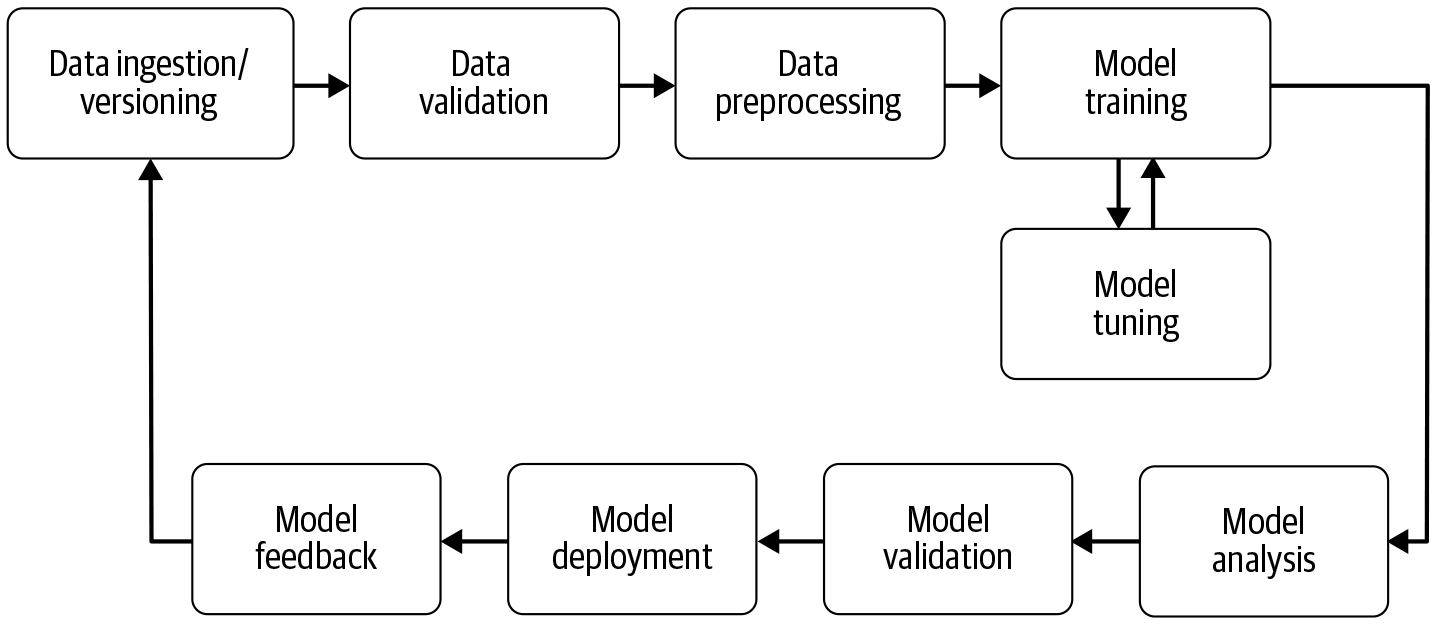
\includegraphics[width=.8\textwidth]{chapter-4/ml-pipeline-lifecycle-oreilly.png}
  \caption{Lifecycle van een model volgens Hapke en Nelson \cite[p.~4]{building-machine-learning-pipelines-oreilly}.}
  \label{fig:model-lifecycle-oreilly}
\end{figure}

In de volgende subkoppen zullen de stappen worden doorlopen met een korte uitleg over wat er gebeurd in een stap. Om een praktisch beeld te schetsen wordt na de uitleg een ML probleem opgelost. Dit wordt gedaan met behulp van de iris dataset in [REFERENCE].

\subsection{Stap 1: Data opname en versiebeheer (Data ingestion/versioning)}\label{subsec:data-opname-en-versiebeheer}
De eerste stap in de pipeline is het opnemen van data. Met deze data zal het model getraind, gevalideerd en getest worden. De dataset kan van een of meerdere bronnen komen, zoals lokaal, een online opslag locatie of van een database. Zodra de data is ingeladen, moet het verdeeld worden tussen een train, validatie en test dataset. Normaal gebeurt dit met een split ratio van 6:2:2. De train dataset is 60\% en de validatie en test datasets zijn allebei 20\% van de originele dataset \cite[p.~27-37]{building-machine-learning-pipelines-oreilly}.

Een use case van een pipeline is dat een nieuw model getraind kan worden door een geüpdatet dataset te gebruiken. Dit wordt gedaan door de voorgaande dataset te gebruiken waarbij nieuwe data is toegevoegd. Door het gebruik van verschillende datasets is het verstandig om versiebeheer toe te passen. Zo is goed te zien welk dataset welk model produceert. Een versie geven aan een dataset gebeurt voordat de dataset wordt ingeladen \cite[p.~39-40]{building-machine-learning-pipelines-oreilly}. Versiebeheer voor datasets kan bijvoorbeeld met DVC \cite{dvc} of Pachyderm \cite{pachyderm}.

% De iris dataset wordt in \autoref{fig:step-1} geïmporteerd door middel van code. Normaal gesproken zou, voordat deze code uitgevoerd wordt, een versie gegeven worden aan de dataset. Omdat de schaal van dit voorbeeld klein is en om de voorbeeld reproduceerbaar te houden is dit niet gedaan. De dataset wordt aangemaakt met de namen voor de kolommen op regel 5 net zoals het voorbeeld in \autoref{table:example-iris-dataset}. Vervolgens is de dataset onder de variabel naam \(dataset\) beschikbaar voor de komende stappen.

% \begin{figure}[hbt!]
%   \centering
%   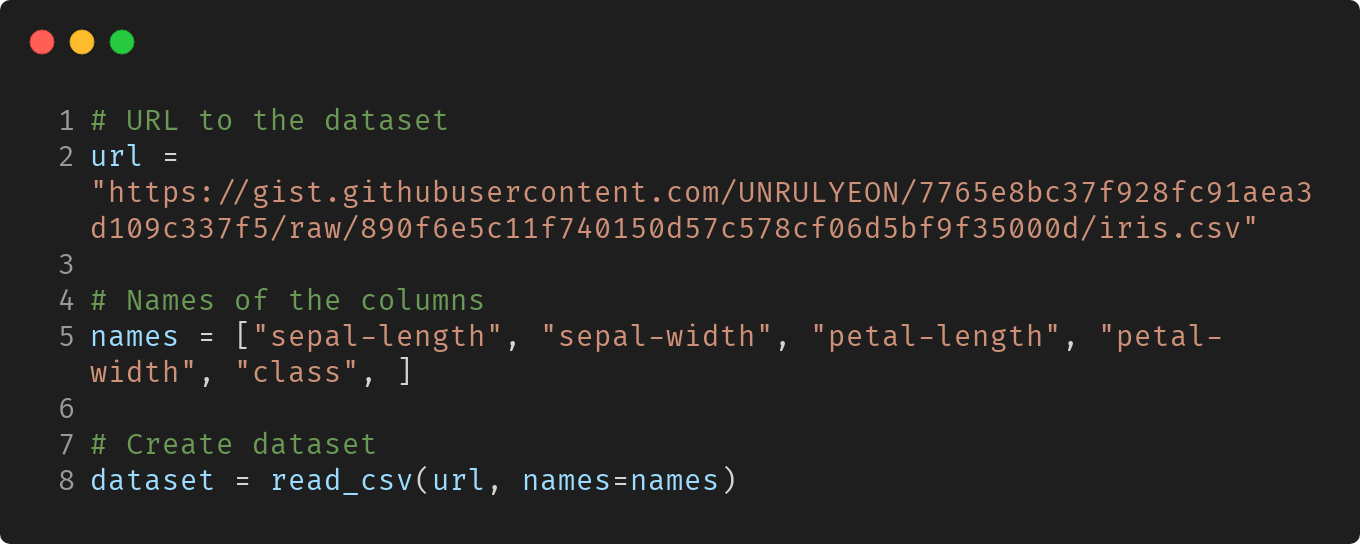
\includegraphics[width=.8\textwidth]{chapter-4/step-1.png}
%   \caption{Dataset importeren}
%   \label{fig:step-1}
% \end{figure}

\subsection{Stap 2: Data validatie (Data validation)}\label{subsec:data-validatie}
Nu de dataset verdeeld is, een versie heeft en op een bereikbare plek is, kan de data gevalideerd worden. Deze stap is vooral belangrijk om te voorkomen dat een model wordt getraind dat niet nuttig is aangezien het trainen veel tijd in beslag kan nemen. Een bekende uitdrukking is "garbage in = garbage out". Dit betekent dat als de dataset niet goed is, het model ook niet goed zal presteren \cite[p.~43]{building-machine-learning-pipelines-oreilly}. Tijdens de validatie stap wordt gecontroleerd op het volgende:

\begin{itemize}
  \item Afwijkingen in de dataset
  \item Wijzigingen in de structuur
  \item Algemene statistieken in vergelijkingen met voorgaand datasets \cite[p.~44]{building-machine-learning-pipelines-oreilly}
\end{itemize}

Bij het controleren van afwijkingen in de dataset wordt gekeken naar waardes die opmerkelijk zijn. Afwijkende waardes liggen te ver van het gemiddelde en kan een verkeerd beeld schetsen bij het trainen van het model. Deze uitschieters kunnen simpelweg uit de dataset gefilterd worden.

Het kan voorkomen dat bij een nieuw dataset de type van waardes zijn gewijzigd. Een \(int\) kan bijvoorbeeld veranderd zijn in een \(string\) of \(boolean\). Er is dan sprake van een wijziging in de structuur van het dataset. Dit is problematisch omdat er een vertaalstap gemaakt moet worden naar iets bruikbaars. Als dit niet mogelijk is moeten de waardes uitgefilterd worden wat de prestatie van het model negatief kan beïnvloeden.

De algemene statistieken is een hulpmiddel om te controleren op afwijkingen en wijzigingen. Vaak kan de controle in een oogopslag gedaan worden. 

% De code voor het genereren van de statistieken hangt af van hoe de dataset eruit ziet en wat er gegenereerd moet worden. In \autoref{fig:step-2} is te zien hoe statistieken worden gegenereerd uit de iris dataset.

% \begin{figure}[hbt!]
%   \centering
%   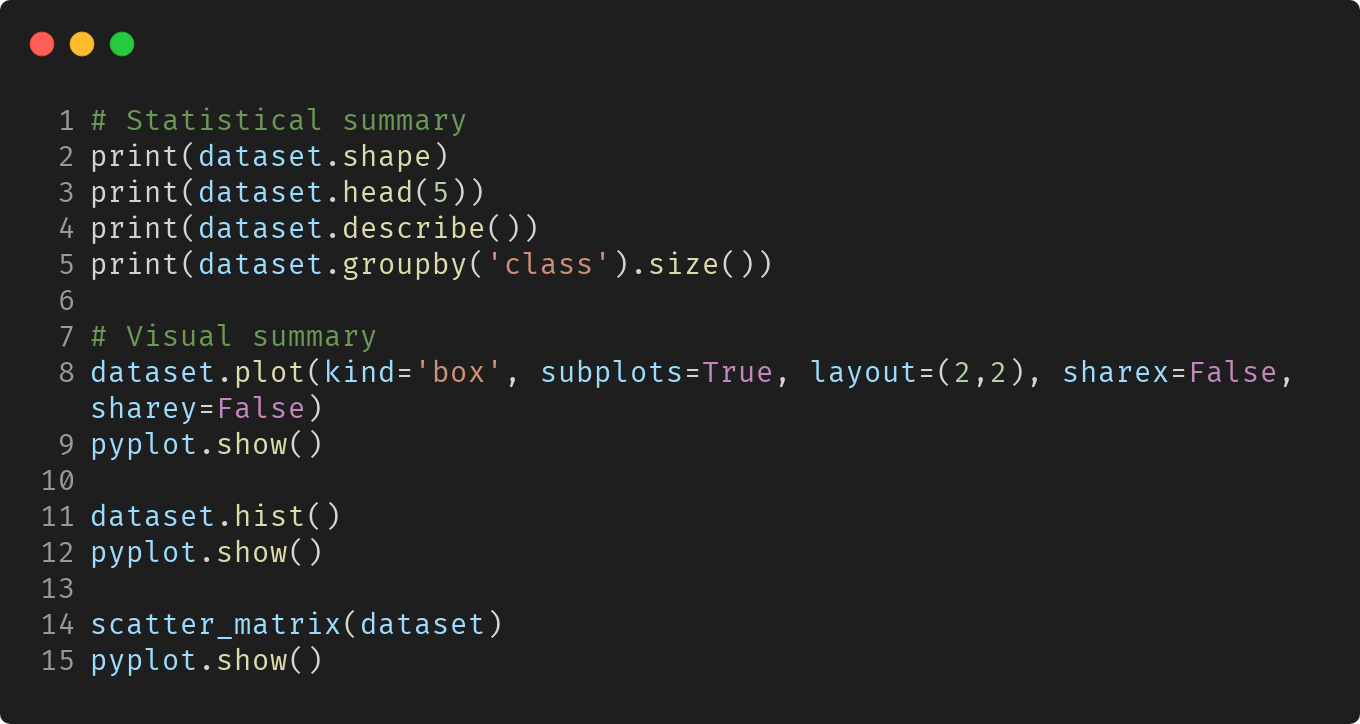
\includegraphics[width=.8\textwidth]{chapter-4/step-2.png}
%   \caption{Statistieken genereren}
%   \label{fig:step-2}
% \end{figure}

% \begin{figure}[hbt!]
%   \centering
%   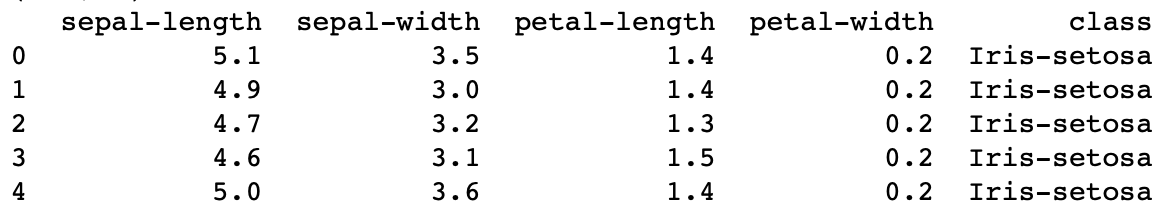
\includegraphics[width=.9\textwidth]{chapter-4/step-2-head-dataset.png}
%   \caption{Statistieken - Eerste 5 regels van de iris dataset}
%   \label{fig:step-2-head-dataset}
% \end{figure}

% \begin{figure}[hbt!]
%   \centering
%   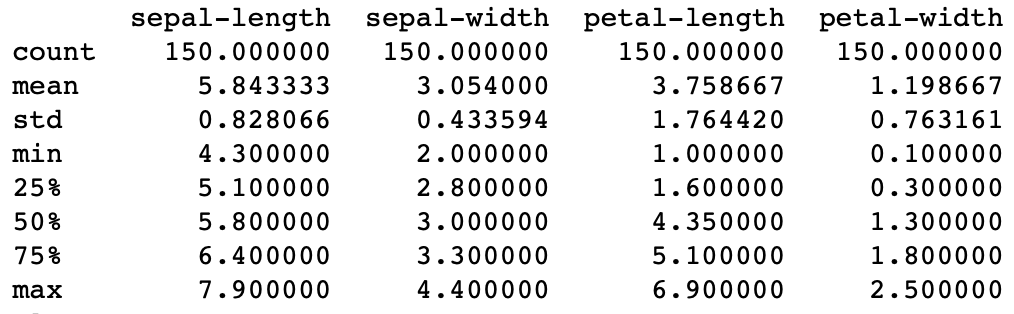
\includegraphics[width=.8\textwidth]{chapter-4/step-2-dataset-described.png}
%   \caption{Statistieken - De iris dataset beschreven}
%   \label{fig:step-2-dataset-described}
% \end{figure}

% \begin{figure}[hbt!]
%   \centering
%   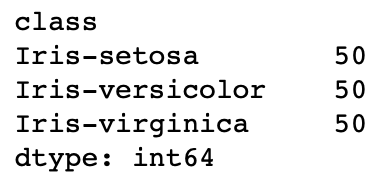
\includegraphics[width=.4\textwidth]{chapter-4/step-2-grouped-by-class.png}
%   \caption{Statistieken - Iris dataset gegroepeerd}
%   \label{fig:step-2-grouped-by-class}
% \end{figure}

\subsection{Stap 3: Data voorbereiden (Data preprocessing)}\label{subsec:data-voorbereiden}
Het voorbereiden van het dataset is een stap dat de prestatie van het model verbetert en het proces van het trainen versneld. Deze stap kan verdeeld worden in twee sub-stappen: het opschonen en het optimaliseren van het dataset.

Bij het opschonen worden bijvoorbeeld duplicaten of waardes die onbruikbaar zijn uit het dataset weggehaald. Onbruikbare waardes zijn waardes die simpelweg niet kloppen of verkeerd zijn ingevoerd. Hierbij kan bijvoorbeeld gedacht worden aan een medewerken die de interactietijd met een klant moet bijhouden, maar is vergeten om de eindtijd te noteren. Voor het algoritme zal het dan lijken alsof de medewerker een klant tot sluitingstijd heeft geholpen.

Datasets kunnen geoptimaliseerd worden om twee redenen: algoritmes werken sneller met waardes die dichter bij \(0\) liggen en algoritmes kunnen niet met elke waarde in het dataset omgaan. Om de efficiëntie van het algoritme te verbeteren kunnen een aantal technieken gebruikt worden:

\begin{itemize}
  \item Schalen
  \item[] Bij het schalen van data worden de waardes getransformeerd waardes dat ligt tussen een schaal, zoals tussen \(0\) en \(100\) of \(0\) en \(1\). Bij het schalen wordt het \textbf{bereik} getransformeerd \cite{scale-and-normalize-data}. 
  \item Normaliseren
  \item[] Als een dataset wordt gestandaardiseerd, worden de waarden getransformeerd in een standaard normale verdeling waarbij het gemiddelde \(0\) en de afwijking \(1\) is. Hierbij wordt de \textbf{vorm} van het dataset getransformeerd \cite{scale-and-normalize-data}. Het normaliseren is belangrijk als het algoritme waardes vergelijkt met verschillende eenheden \cite{feature-scaling-standardization}. In sommige gevallen is normalisering een vereiste bij een aantal algoritmes \cite{data-transformation-standardization-vs-normalization}.
  \item Categorisch codering
  \item[] Een groot aantal algoritmes kan alleen omgaan met numerieke waardes. Het kan voorkomen data datasets categorische waardes bevatten. Dit zijn waardes dat een label voorstellen, zoals \(cat\) of \(dog\). Om deze waardes te gebruiken moeten ze worden gecodeerd als een numerieke waarde. De label kan als de waarde \(1\) of \(2\) gecodeerd worden. Deze techniek heet integer encoding. Een andere techniek om waardes te coderen heet hot encoding. Deze techniek maakt gebruikt van meerdere waardes om een label te beschrijven.
\end{itemize}

%\begin{matrix}
%  cat & dog & mouse\\
%  1 & 0 & 0
%  0 & 1 & 0
%  0 & 0 & 1
%\end{matrix} 

Na het opschonen en optimaliseren kan het dataset gebruikt worden om een model te trainen. Dit is een goed moment om het getransformeerde dataset op te slaan als "tussen-dataset" zodat deze stap niet herhaalt hoeft te worden. Het voorbereiden van grote datasets kan een grote hoeveelheid tijd in beslag nemen.

\subsection{Stap 4 en 5: Model trainen en tunen (Model training and Model tuning)}\label{subsec:model-trainen-en-tunen}


Een ML algoritme is vergelijkbaar met een conventionele algoritme in software engineering. Het algoritme slaat na het trainen met een dataset de regels, nummers en algoritme specifieke data structuren op in de vorm van een model. Het model is als het ware een programma waarmee, gegeven een input, voorspellingen mee gedaan kan worden [https://machinelearningmastery.com/difference-between-algorithm-and-model-in-machine-learning/].



Een algoritme is geoptimaliseerd om een specifieke taak te doen, zoals het voorspellen van woorden of voorwerpen in een afbeelding herkennen. Een mindmap met algoritmes is te vinden in [BIJLAGE]. Zo is goed te zien hoeveel algoritmes hetzelfde bereiken. Hierom is het verstandig om vooraf te testen welke het beste werkt voor het gegeven ML probleem.

Over het algemeen gebeurt er hetzelfde, ongeacht welk algoritme is gebruikt [p84]:

\begin{itemize}
  \item Laad de train en validatie dataset
  \item Definieer het model
  \item Train het model
  \item Sla het model op
\end{itemize}

[Hyperparameters uitleg]

[Uitleg hyperparameters SVC] [https://scikit-learn.org/stable/modules/generated/sklearn.svm.SVC.html]

\subsection{Stap 6 en 7: Model analyse en validatie (Model analysis and Model validation)}\label{subsec:model-analyse-en-validatie}
De prestatie valideren en vergelijken met voorgaande modellen is het analyseren. 

Ethische verantwoording van het model is validatie. Waarom het belangrijk is om het model te analyseren. Hoe behandeld het model voorspellingen van:

\begin{itemize}
  \item mensen met verschillende variabelen zoals geslacht, locatie of leeftijd.
  \item image recognition met verschillende licht condities.
\end{itemize}

Meetinstrumenten voor algoritme groepen.

Voor voorbeeld kan classification metrics (confusion matrix) gebruikt worden.

\subsection{Stap 8: Model uitrollen (Model deployment)}\label{subsec:model-uitrollen}
Het opgeslagen model kan simpelweg geladen worden in een webserver zoals Flask. Dit schaalt echter niet en het is lastig om bij te houden met welke versie van het model een voorspelling wordt gedaan.

Tensorflow Serving maakt dit makkelijker. Korte uitleg hoe TS Serving dit makkelijker maakt. Eventueel andere oplossingen

\subsection{Stap 9: Feedback loop (Model feedback)}\label{subsec:feebdack-loop}
Impliciet en expliciet feedback

\begin{itemize}
  \item Impliciet
  \item [] Een gebruiker kijkt een gesuggereerde film of koopt een gesuggereerde item in een webshop.
  \item Expliciet
  \item [] De applicatie vraagt aan de gebruiker of de suggestie waarde heeft.
\end{itemize}

[REFERENCE]

\subsection{De machine learning pipeline toegepast op een probleem}\label{subsec:de-machine-learning-pipeline-toegepast-op-een-probleem}
\begin{itemize}
  \item Om een beeld te geven van de ML pipeline wordt een ML probleem opgelost
  \item Het probleem is een bekend probleem binnen het ML domein omdat de focus op de pipeline ligt en niet of het ML probleem opgelost kan worden of niet
  \item Het probleem is gekozen omdat het een bekend probleem is binnen het ML domein en het doel is om de stappen in de ML pipeline te beproeven en niet om te experimenteren met onopgeloste problemen.
  \item Het doel is om een ML model te trainen dat, aan de hand van de afmetingen van de kelk- en bloemblad, kan identificeren tot welke familie een iris bloem hoort.
  \item Uitleg dataset \autoref{table:example-iris-dataset}
\end{itemize}

\begin{table}[hbt!]
  \footnotesize
  \centering
  \begin{tabular}{|l|l|l|l|l|}
  \hline
  \textbf{Kelkblad - lengte} & \textbf{Kelkblad - breedte} & \textbf{Bloemblad - lengte} & \textbf{Bloemblad - breedte} & \textbf{Soort} \\ \hline
  5.1 & 3.5 & 1.4 & 0.2 & Iris-setosa\\ \hline
  \end{tabular}
  \caption{Voorbeeld van de iris dataset}
  \label{table:example-iris-dataset}
\end{table}

\section{Conclusie}\label{conclusie}
\begin{itemize}
  \item Een ML pipeline is een manier om gestructureerd en reproduceerbaar een ML model te trainen
  \item Er is geen consensus over wat de stappen in een ML pipeline zijn
  \item Gedurende de pipeline wordt er gefocust op de kwaliteit van de dataset en prestatie van het model
\end{itemize}

\section{Advies}\label{advies}
\begin{itemize}
  \item Het opzetten van een pipeline neemt tijd in beslag, maar het is het waard op de lange termijn
  \item Door de gestructureerde werkwijze is het goed bij te houden hoe het model tot stand is gekomen
  \item 
\end{itemize}

% \subsection{Praktisch voorbeeld: iris dataset}\label{subsec:de-stappen-met-een-praktisch-voorbeeld}


% Het praktisch voorbeeld is een ML pipeline dat geschreven is in Python en lokaal gedraaid kan worden. Niet alle stappen kunnen worden vertaalt naar de lokale ML pipeline. Dit zal worden aangegeven bij de stappen in kwestie.
